\section{Figures}
% Expect: this section comes from chapters/figures.tex through \include.

\subsection{Images}
% Expect: the same four-color image, first full size with a caption under it.
% The image comes from figures/quadrants.png in the file tree.
\begin{figure}
  \centering
  
\includegraphics{figures/quadrants.png}
  \caption{A project image, full size.}
\end{figure}

\subsubsection{Image sizes}
% Expect: an image half as wide as the text column.

\includegraphics[width=0.5\textwidth]{figures/quadrants}

% Expect: an image 2cm wide (about 76px), with its height kept in proportion.

\includegraphics[width=2cm]{figures/quadrants}

% Expect: an image 1in tall (96px), with its width kept in proportion.

\includegraphics[height=1in]{figures/quadrants}

% Expect: an image stretched to 4cm wide and 1cm tall.

\includegraphics[width=4cm,height=1cm]{figures/quadrants}

% Expect: an image fitted inside 4cm by 1cm without stretching, so it is 1cm tall.

\includegraphics[width=4cm,height=1cm,keepaspectratio]{figures/quadrants}

% Expect: an image at half its natural size (48px by 32px).

\includegraphics[scale=0.5]{figures/quadrants}

\subsection{PDF and EPS figures}
% Expect: a bar chart (red, green and blue bars on axes, "PDF figure p1" at the top) at its
% natural size, 2in by 1.33in. It comes from page 1 of figures/chart.pdf, drawn with pdf.js.
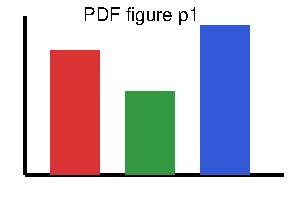
\includegraphics{figures/chart.pdf}

% Expect: page 2 of the same PDF, a blue diamond with "page 2" on it, 3cm wide.
\includegraphics[page=2,width=3cm]{figures/chart}

% Expect: only the right-hand blue bar of page 1, cut out with trim and clip, 1in tall.
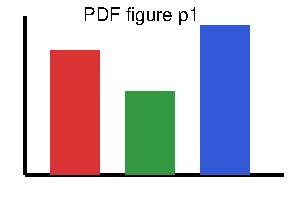
\includegraphics[trim=90bp 8bp 18bp 11bp,clip,height=1in]{figures/chart.pdf}

% Expect: a dashed box 2in by 1in (the file's %%BoundingBox) with the name figures/wave.eps
% and "EPS can't be previewed; convert it to PDF." in it. The ⓘ list says EPS figures show as boxes.

\includegraphics{figures/wave.eps}

% Expect: the same EPS box at half the column width, keeping its 2:1 shape.

\includegraphics[width=0.5\textwidth]{figures/wave}

\subsection{Pictures}
% Expect: a box with a line across it and a circle in the middle.
% A picture compiles on the main thread instead of the worker, since LaTeX.js needs the real DOM to size it.
\setlength{\unitlength}{1mm}
\begin{picture}(40,20)
  \put(0,0){\framebox(40,20){}}
  \put(0,0){\line(2,1){40}}
  \put(20,10){\circle{8}}
\end{picture}
